\documentclass[notitlepage, 12pt]{article}
\usepackage[english]{babel}           % LANGEUAGE=ENGLISH, UTF-8
\usepackage[utf8]{inputenc}
\usepackage[T1]{fontenc}
\usepackage{amsmath}                  % ALL MATH FEATURES
\usepackage{graphicx}                 % GRAPHICS                  
\usepackage{float}                    % IMPROVED FIGURE POSITIONING
\usepackage[labelsep=period,labelfont=bf]{caption} % IMPROVED CAPTIONS
\usepackage{url}                      % WRITE URLS
\usepackage{tikz}                     % MAKE TIKZ VECTOR GRAPHICS
\usepackage{tocloft}                  % CONTROL TABLE OF CONTENTS
\usepackage[authoryear,round]{natbib} % REFERENCES
\usepackage{apalike}
\usepackage{pdflscape}                % USE LANDSCAPE MODE
\usetikzlibrary{decorations.pathreplacing}

\renewcommand{\familydefault}{lmr}           % SET DOCUMENT FONT
\makeatletter                         
\renewcommand{\section}{\@startsection       % SECTION
        {section}
        {2ex}
        {0mm}
        {1.2\baselineskip}
        {\baselineskip}
        {\centering\normalsize}}
\renewcommand{\subsection}{\@startsection    % SUBSECTION
        {subsection}
        {2ex}
        {0mm}
        {.8\baselineskip}
        {.5\baselineskip}
        {\bfseries\normalsize}}
\renewcommand{\subsubsection}{\@startsection % SUBSUBSECTION
        {subsubsection}
        {2ex}
        {0mm}
        {.5\baselineskip}
        {0mm}
        {\it\bfseries\normalsize}}    
\makeatother

% define algorithm environments
\floatstyle{plaintop}
\newfloat{algorithm}{bpht}{alg}
\floatname{algorithm}{Algortihm}

%define title matter
\title{Simulating a dark matter halo using a parallel grid method}
\author{{\em Otto Hannuksela} \and {\em Janne Lampilahti}}
\date{\today}

\begin{document}
\maketitle
\section*{INTRODUCTION}
Dark matter appears to be the dominant form of matter in the universe. While no direct observations of dark matter exist, it has been observed indirectly through its gravitational interaction with visible matter and radiation \citep{Roos2010}. The effect of dark matter on structure formation in the universe is the subject of an increasing scientific interest and a useful tool in the search for possible candidates of dark matter. Current progress in the investigation of structure formation is mainly driven by advances in computational methods and capabilities \citep{Kuhlen2012}. 

In this work we simulate a dark matter halo, neglecting baryonic matter, by using a particle based method and solving the Poisson's equation of gravity. The software used is {\em Uintah} available from \url{http://uintah.utah.edu/}, a parallel grid framework with a support for particle interactions and adaptive mesh refinement and which is aimed at solving partial differential equations.

\section*{METHODS}

%%%%%
\subsection*{Theory}
A distribution of mass density $\rho$ gives rise to a gravitational potential $\phi$ according to the Poisson's equation of gravity
\begin{equation}
\nabla^2 \phi = 4\pi G \rho,
\end{equation}
where $G\approx 6.674\times10^{-11}$ Nm$^2$/kg$^2$ is the gravitational constant. The corresponding force field can be solved from the gradient
\begin{equation}
\mathbf{F} = -\nabla \phi.
\end{equation}
In our simulation a distribution of massive particles create the mass density. A new position and velocity for the particles after a time step $dt$ can be solved from the Newton's equation of motion.
\begin{align}
\mathbf{v}(t+dt) &= \int_{t}^{t+dt}\frac{\mathbf{F}(t')}{m}dt' +  \mathbf{v}(t)\\
\mathbf{x}(t+dt) &= \int_{t}^{t+dt}\mathbf{v}(t')dt' +  \mathbf{x}(t)
\end{align}
The use of this theory assumes that we do not have relativistic speeds or masses and that the maximum grid size is small enough that expansion of the universe can be neglected.  

%%%%%
\subsection*{Numerical methods}
The simulation is set up with respect to a three dimensional grid that supports particles (Fig. \ref{fig:grid}).
\begin{figure}[H]
\centering
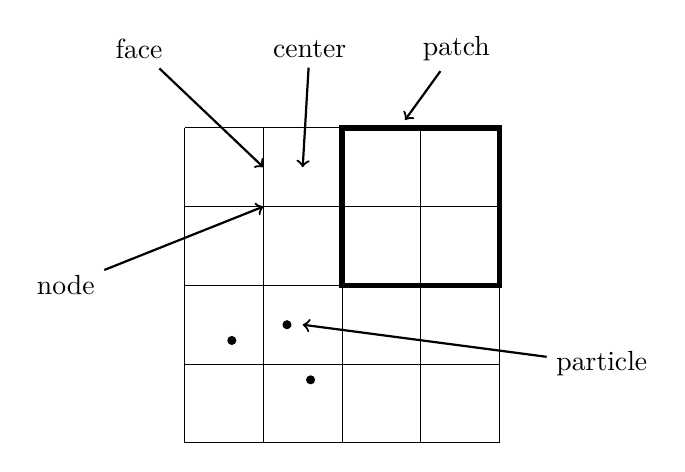
\begin{tikzpicture}
\node [anchor=west] (node) at (-1,3) {node};
\node [anchor=west] (face) at (0,6) {face};
\node [anchor=west] (center) at (2,6) {center};
\node [anchor=east] (patch) at (5,6) {patch};
\node [anchor=east] (particle) at (7,2) {particle};
\draw (1,1) grid (5,5);
%\draw [step=0.5] (3,3) grid (5,5);
%\draw [step=0.1] (4,4) grid (5,5);
\draw [line width=2] (3,3) rectangle (5,5);
\draw [->,thick] (node) -- (2,4);
\draw [->,thick] (face) -- (2,4.5);
\draw [->,thick] (center) -- (2.5,4.5);
\draw [->,thick] (patch) -- (3.8,5.1);
\draw [->,thick] (particle) -- (2.5,2.5);
\draw [fill] (2.3,2.5) circle [radius=0.05];
\draw [fill] (2.6,1.8) circle [radius=0.05];
\draw [fill] (1.6,2.3) circle [radius=0.05];
%\draw [black,decorate,decoration={brace,amplitude=5pt},
%   xshift=5pt,yshift=0pt] (5,5)  -- (5,3)
%   node [black,midway,below=-8pt,xshift=20pt] {AMR};
\end{tikzpicture}
\caption{A two dimensional view of the grid with its various components and properties shown.}
\label{fig:grid}
\end{figure}
The overall algortihm is expressed in Algortihm \ref{alg:main}.
\begin{algorithm}[H]
\hspace{0.1\textwidth}\parbox{.8\textwidth}{
\-\hspace{0ex}set Dirichlet boundary conditions: $\phi=0$\\
\-\hspace{0ex}set initial $\mathbf{x}_p$, $\mathbf{v}_p$ and $m_p$ for all particles $p$\\
\-\hspace{0ex}calculate initial $\rho$\\
\-\hspace{0ex}set initial guess for $\phi$\\
\-\hspace{0ex}{\bf loop}\\
\-\hspace{4ex}solve $\phi$ using SOR algorithm\\
\-\hspace{4ex}calculate $\mathbf{F}=-\nabla \phi$\\
\-\hspace{4ex}{\bf for} every particle $p$ {\bf do}\\
\-\hspace{8ex}$\mathbf{v}_p(t+\Delta t) = (\mathbf{F}_p/m)\Delta t + \mathbf{v}_p(t)$\\
\-\hspace{8ex}$\mathbf{x}_p(t+\Delta t) = \mathbf{v}_p(t)\Delta t + \mathbf{x}_p(t)$\\
\-\hspace{4ex}{\bf end for}\\
\-\hspace{4ex}calculate $\rho$\\
\-\hspace{4ex}$t\leftarrow t+\Delta t$\\
\-\hspace{0ex}{\bf end loop}}
\caption{Main program.}
\label{alg:main}
\end{algorithm}

The Poisson's equation is solved with the successive over relaxation (SOR) algortihm (Algorithm \ref{alg:SOR}). The potential $\phi$ is solved at each node. In the calculation of the potential gradient we obtain the potential values near the particles by interpolation and then calculate the gradient by numerical differentiation. For exmaple at the $p$th particle the gradient is calculated in the $x$ direction as
\begin{equation}
(\nabla \phi)(x_p)=\frac{\phi(x_p+dx)-\phi(x_p-dx)}{2dx},
\end{equation}
where $x_p$ is the particle's $x$ coordinate and $dx$ is a small distance. 

The particle velocity and position are evolved over a small time step $dt$, assuming that the force remains constant. After this the particle masses are again interpolated back to the nodes to obtain a new mass density $\rho$.

\begin{algorithm}[H]
\hspace{0.1\textwidth}\parbox{.8\textwidth}{
\-\hspace{0ex}{\bf function} SOR($\phi$, tolerance, max\_iterations)\\
\-\hspace{4ex}{\bf for} $n = 0,1,\ldots\mbox{max\_iterations}$ {\bf do}\\
\-\hspace{8ex}error $\sigma\leftarrow 0$\\
\-\hspace{8ex}{\bf for} every node $\phi_{i,j,k}$\\
\-\hspace{12ex}$\phi_{i,j,k}^{(n+1)} \leftarrow (1-\omega)\phi_{i,j,k}^{(n)} + \frac{\omega}{6} (\phi_{i+1,j,k}^{(n)} +\phi_{i-1,j,k}^{(n)}+$\\
\-\hspace{12ex}$\phantom{\phi_{i,j,k}^{(n+1)} \leftarrow }\phi_{i,j+1,k}^{(n)}+ \phi_{i,j-1,k}^{(n)} + \phi_{i,j,k+1}^{(n)} + \phi_{i,j,k-1}^{(n)} +$\\
\-\hspace{12ex}$\phantom{\phi_{i,j,k}^{(n+1)} \leftarrow} h^3\rho_{i,j,k})$\\
\-\hspace{12ex}update $\sigma$\\
\-\hspace{8ex}{\bf end for}\\
\-\hspace{8ex}{\bf if} $\sigma \leq $ tolerance, {\bf break}\\
\-\hspace{4ex}{\bf end for}\\
\-\hspace{4ex}{\bf return} $\phi$\\
\-\hspace{0ex}{\bf end function}}
\caption{Calculating potential $\phi$ using the SOR algorithm.}
\label{alg:SOR}
\end{algorithm}

%%%%%
\subsection*{Initialization of the simultaion}
The specific case we want to study with our simulation is a dark matter halo. Dark matter halos are structures composed of dark matter, believed to envelope galaxy disks. We initialize the halo by letting a sphere of randomly distributed dark matter particles to collapse by the effect of gravity.

%%%%%
\subsection*{Verification of results}
To verify the simulation results we test for energy conservation, compliance with the virial theorem 
\begin{equation}
\langle T \rangle_t = -\frac{1}{2}\langle V \rangle_t.
\end{equation}

Previous $N$-body simulations suggest that dark matter halos follow the Navarro-Frenk-White radial mass distribution 
\begin{equation}
\rho(r) = \frac{\rho_0}{\frac{r}{R_s}\left(1 + \frac{r}{R_s}\right)^2},
\end{equation}
where $r$ is distance from the center of the halo and $(\rho_0,R)$ are parameters. As part of our verification procedure we fit this distribution to the simulated dark matter halo.

\section*{IMPLEMENTATION}
\subsection*{Uintah}
% describe uintah
\subsection*{The program}
\section*{RESULTS}
% visit figure:
% initial vs final condition
% mp4 movie...
\section*{CONCLUSIONS}
% what should we do next?

%\renewcommand{\refname}{REFERENCES} 
%\bibliography{NameOfReferenceFile}{}
%\bibliographystyle{plainnat}
\end{document}
